% ¿Qué son las metodologías ágiles?
Las metodologías ágiles nos permiten una mayor flexibilidad que las metodologías tradicionales de desarrollo, que debido a una mayor rigidez en sus procesos y en la documentación no nos permiten ajustarnos a cambios que pueden producirse en las necesidad del cliente, en el mercado o en desafíos que pueda plantearnos las tecnologías que planeamos emplear. Además exísteme determinadas metodologías probadas y centradas para el desarrollo de aplicaciones móviles. A continuación se procede a explicar en qué consisten las metodologías ágiles y a hablar de la metodología \textit{Mobile-D}, escogida para la realización de dicho proyecto.

\subsubsection*{Metodologías ágiles}
En el año 2001 se celebró una reunión en Utah de la cual surgió el término ``ágil'' aplicado al desarrollo de software. El objetivo de dicha reunión fue establecer principios y valores que permitirían a equipos de desarrollo agilizar y responder a todo los cambios que surgen en los proyectos. Estos "métodos ágiles" se plantean como una alternativa a las metodologías convencionales más rígidas y centradas en la documentación que se genera tras cada actividad. \\

Las motivaciones principales que llevan a estas nuevas metodologías tratan de dar solución a dos problemáticas: por un lado el alto porcentaje de proyectos que fracasan o se retrasan; y por otro la baja calidad de estos\cite{metodologidesarrollo2009}. \\

\subsubsection*{Mobile-D}
% ¿Qué es?
Dentro de las metodologías ágiles, Mobile-D es una creada por el VTT\footnote{Technical Research Centre of Finland} en colaboración estrecha con la industria de TI finlandesas. Se desarrolla en el año 2004 para un proyecto finlandés llamado ICAROS. Esta metodología se crea centrándose en el desarrollo de aplicaciones móviles. Cabe destacar que los autores consideraron dos aspectos: por un lado equipos pequeños de 10 personas o menos, y por otro la disposición de proyectos funcionales en menos de 10 semanas. Todo ello lo hace idóneo para el desarrollo de aplicaciones móviles \cite{metodologidesarrollo2009}. \\
Esta metodología es una mezcla de técnicas utilizadas por otras metodologías ágiles tales como \textit{eXtreme Programming},\textit{Crystal methodologies} y \textit{Rational Unified Process}. De la \textit{eXtreme Programming} se emplean prácticas de desarrollo, \textit{Crystal metodologies} proporciona inputs importantes en lo referidos a escalabilidad de los métodos; y de \textit{Rational Unified Process} se toman las bases para el diseño completo del ciclo de vida. \\
% Fases
Para la planificación de dicha metodología se establecen cinco fases. A excepción de la fase inicial, en cada una de las fases se establece un día de planificación y uno de entrega. Las fases \cite{AgileMobileD} se muestran en el siguiente gráfico:
\begin{figure}[H]
\centering
    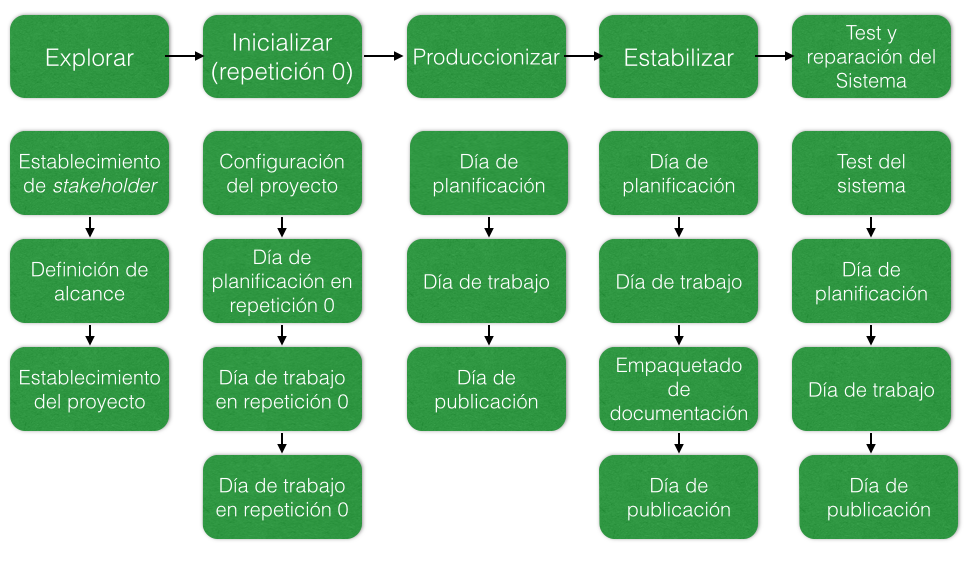
\includegraphics[scale=0.35]{etapasmobile-d.png}
    \caption{Fases de la metodología Mobile-D}
\end{figure}
% Se enumeran las fases de la metodología
\begin{itemize}
    \item \textbf{Exploración: }el propósito de dicha fase es planificar y establecer el inicio del proyecto. Se establecen los \textit{stakeholders}, se definen los objetivos y se lleva a cabo la planificación del proyecto.
    \item \textbf{Inicialización: }se identifican los recursos necesarios, se establece el entorno de desarrollo y la formación inicial.
    \item \textbf{Productización: }en esta fase se realiza una repetición iterativa de subfases. Se emplean técnicas de \textit{test driven development} para el desarrollo.
    \item \textbf{Estabilización: }se procede a la integración de todas las partes del sistema.
    \item \textbf{Test y reparación del sistema: }se prueba el sistema según los requisitos establecidos, se llevan a cabo correcciones y finalmente se obtiene una versión estable y funcional.
\end{itemize}